
\documentclass{ximera}

\usepackage[a4paper,left=1.5cm,right=1.5cm]{geometry}
\usepackage{amsmath}
\usepackage{amssymb}
\usepackage{ifthen}
\usepackage{environ}
\usepackage{multicol}
\usepackage{tikz} 
\usepackage{pgfplots} 
\usepackage{enumitem}
\pgfplotsset{compat=1.18}

\renewenvironment{exercise}[1][2in]
{
    \stepcounter{problem@Depth}
    \begin{trivlist}
    \item[\normalfont\bfseries Oefening\hspace{0.2em}\problemNumber)]
    \leavevmode\par
    \normalfont
}
{
    \problemEnvironmentEnd
}

\renewenvironment{solution}
{
    \ifhandout
        \setbox0\vbox\bgroup
    \else
        \begin{trivlist}
        \item[\normalfont\bfseries Oplossing:]
        \leavevmode\par
        \normalfont
    \fi
}
{
    \ifhandout
        \egroup
    \else
        \end{trivlist}
    \fi
}

\renewenvironment{question}
{
    \stepcounter{problem@Depth}
    \begin{trivlist}
    \item[\normalfont\bfseries Vraag\hspace{0.2em}\problemNumber)]
    \leavevmode\par
    \normalfont
}
{
    \problemEnvironmentEnd
}

\usepackage{fancyhdr}

\pagestyle{fancy}
\fancyhf{}

% Left footer
\fancyfoot[L]{%
    \small Monitoraat geneeskunde
}

% Right footer
\fancyfoot[R]{%
    \small
    Bij vragen: \texttt{arne.vandamme@kuleuven.be}
}

% Footer styling
\renewcommand{\headrulewidth}{0pt}
\renewcommand{\footrulewidth}{0.4pt}

% Apply identical footer to plain pages (e.g. first page)
\fancypagestyle{plain}{%
    \fancyhf{}
    \fancyfoot[L]{\small Monitoraat Geneeskunde}
    \fancyfoot[R]{%
        \small
        Bij vragen: \texttt{arne.vandamme@kuleuven.be}
    }
    \renewcommand{\headrulewidth}{0pt}
    \renewcommand{\footrulewidth}{0.4pt}
}

\usepackage{graphicx}


\begin{document}

\begin{center}
    {\Large\textbf{Fasediagram van water}}
\end{center}

\medskip

\begin{exercise}

Wat gebeurt er als we de druk verlagen bij constante temperatuur, vanuit een toestand van $218\,\text{atm}$ en $-1\,^\circ\text{C}$?

\bigskip

\begin{center}
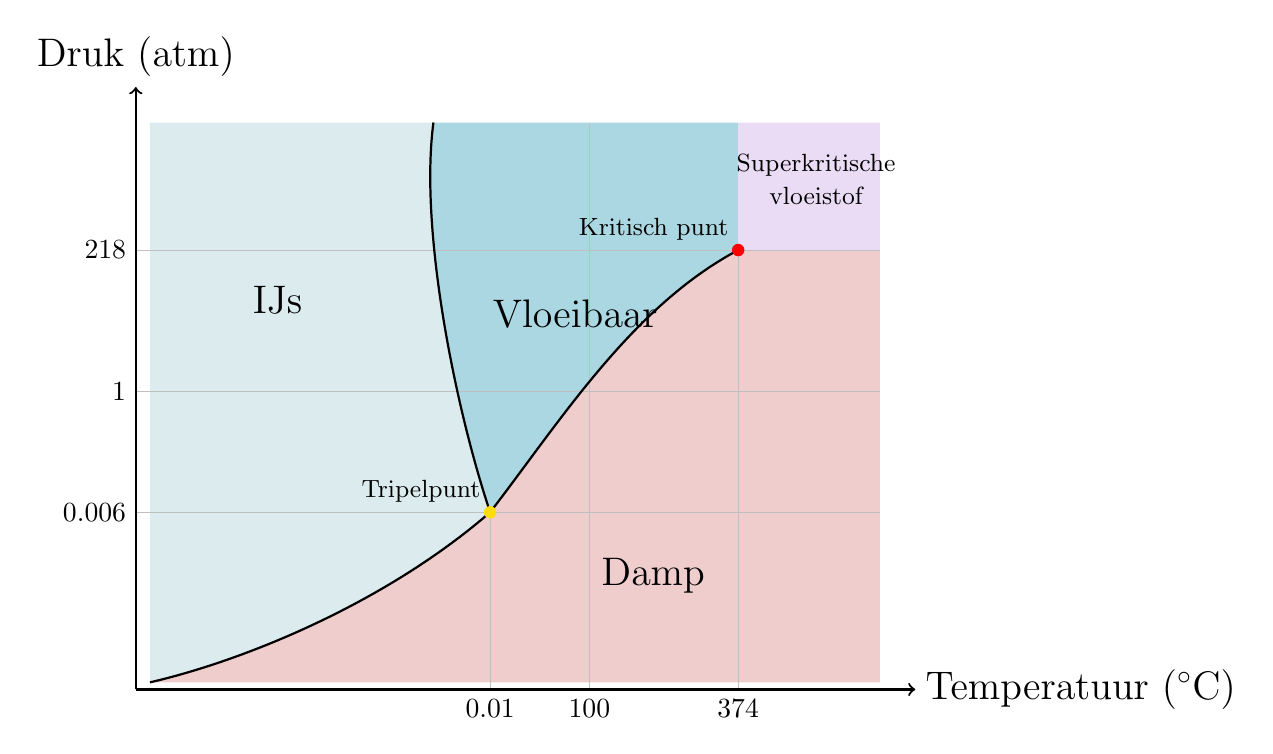
\begin{tikzpicture}[scale=0.9]

% Kleuren
\definecolor{icecol}{RGB}{220,235,238}
\definecolor{watercol}{RGB}{170,215,225}
\definecolor{steamcol}{RGB}{240,205,205}
\definecolor{supercol}{RGB}{235,220,245}

% Referentiepunten
\coordinate (T) at (5,2.5);
\coordinate (C) at (8.5,6.2);

% Stoomgebied
\fill[steamcol]
    (0.2,0.1)
    .. controls (1.5,0.4) and (3.5,1.2) .. (T)
    .. controls (6.0,3.8) and (7.0,5.4) .. (C)
    -- (10.5,6.2)
    -- (10.5,0.1)
    -- cycle;

% IJsgebied
\fill[icecol]
    (0.2,8)
    -- (4.2,8)
    .. controls (4.0,6.5) and (4.5,4.0) .. (T)
    .. controls (3.5,1.2) and (1.5,0.4) .. (0.2,0.1)
    -- cycle;

% Watergebied
\fill[watercol]
    (T)
    .. controls (4.5,4.0) and (4.0,6.5) .. (4.2,8)
    -- (8.5,8)
    -- (C)
    .. controls (7.0,5.4) and (6.0,3.8) .. (T)
    -- cycle;

% Superkritisch gebied
\fill[supercol]
    (C)
    -- (10.5,6.2)
    -- (10.5,8)
    -- (8.5,8)
    -- cycle;

% Hulplijnen
\draw[gray!50] (0,2.5) -- (10.5,2.5);
\draw[gray!50] (0,4.2) -- (10.5,4.2);
\draw[gray!50] (0,6.2) -- (10.5,6.2);

\draw[gray!50] (5,0) -- (5,2.5);
\draw[gray!50] (6.4,0) -- (6.4,8);
\draw[gray!50] (8.5,0) -- (8.5,6.2);

% Fasegrenzen
\draw[thick]
    (0.2,0.1)
    .. controls (1.5,0.4) and (3.5,1.2) .. (T);

\draw[thick]
    (4.2,8)
    .. controls (4.0,6.5) and (4.5,4.0) .. (T);

\draw[thick]
    (T)
    .. controls (6.0,3.8) and (7.0,5.4) .. (C);

% Assen
\draw[->,thick] (0,0) -- (11,0)
    node[right] {\Large Temperatuur ($^\circ$C)};

\draw[->,thick] (0,0) -- (0,8.5)
    node[above] {\Large Druk (atm)};

% Tripelpunt
\fill[yellow!80!orange] (T) circle (2.5pt);
\node[above left] at (T) {\small Tripelpunt};

% Kritisch punt
\fill[red] (C) circle (2.5pt);
\node[above left] at (C) {\small Kritisch punt};

% Gebiedslabels
\node at (2.0,5.5) {\Large IJs};
\node at (6.2,5.3) {\Large Vloeibaar};
\node at (7.3,1.6) {\Large Damp};

\node[align=center] at (9.6,7.2) {
    \small Superkritische\\
    \small vloeistof
};

% y-ticks
\node[left] at (0,2.5) {0.006};
\node[left] at (0,4.2) {1};
\node[left] at (0,6.2) {218};

% x-ticks
\node[below] at (5,0) {0.01};
\node[below] at (6.4,0) {100};
\node[below] at (8.5,0) {374};

\end{tikzpicture}
\end{center}

\bigskip

\begin{solution}

Bij een druk van $218\,\text{atm}$ en een temperatuur van $-1\,^\circ\text{C}$ bevindt water zich in de vloeibare fase.

We verlagen de druk terwijl de temperatuur constant blijft op $-1\,^\circ\text{C}$. In het fasediagram bewegen we dus verticaal naar beneden.

\begin{center}
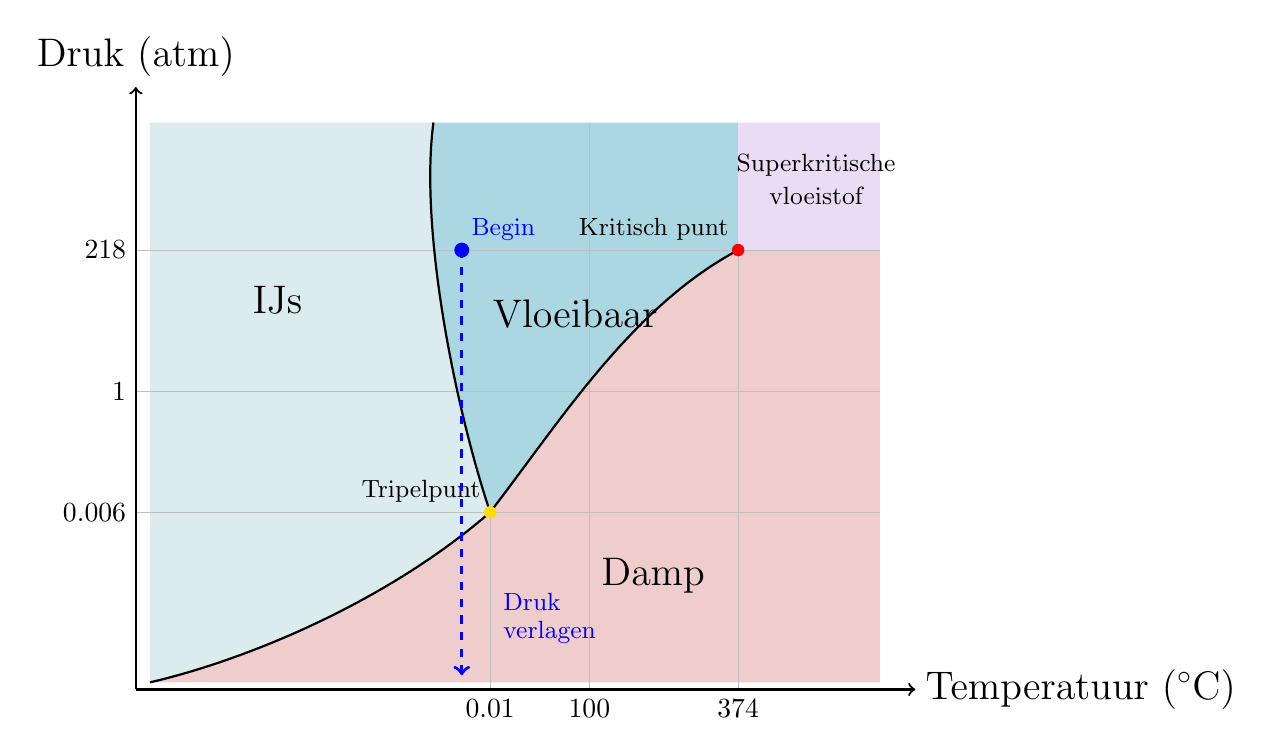
\begin{tikzpicture}[scale=0.9]

% Kleuren
\definecolor{icecol}{RGB}{220,235,238}
\definecolor{watercol}{RGB}{170,215,225}
\definecolor{steamcol}{RGB}{240,205,205}
\definecolor{supercol}{RGB}{235,220,245}

% Referentiepunten
\coordinate (T) at (5,2.5);
\coordinate (C) at (8.5,6.2);

% Stoomgebied
\fill[steamcol]
    (0.2,0.1)
    .. controls (1.5,0.4) and (3.5,1.2) .. (T)
    .. controls (6.0,3.8) and (7.0,5.4) .. (C)
    -- (10.5,6.2)
    -- (10.5,0.1)
    -- cycle;

% IJsgebied
\fill[icecol]
    (0.2,8)
    -- (4.2,8)
    .. controls (4.0,6.5) and (4.5,4.0) .. (T)
    .. controls (3.5,1.2) and (1.5,0.4) .. (0.2,0.1)
    -- cycle;

% Watergebied
\fill[watercol]
    (T)
    .. controls (4.5,4.0) and (4.0,6.5) .. (4.2,8)
    -- (8.5,8)
    -- (C)
    .. controls (7.0,5.4) and (6.0,3.8) .. (T)
    -- cycle;

% Superkritisch gebied
\fill[supercol]
    (C)
    -- (10.5,6.2)
    -- (10.5,8)
    -- (8.5,8)
    -- cycle;

% Hulplijnen
\draw[gray!50] (0,2.5) -- (10.5,2.5);
\draw[gray!50] (0,4.2) -- (10.5,4.2);
\draw[gray!50] (0,6.2) -- (10.5,6.2);

\draw[gray!50] (5,0) -- (5,2.5);
\draw[gray!50] (6.4,0) -- (6.4,8);
\draw[gray!50] (8.5,0) -- (8.5,6.2);

% Fasegrenzen
\draw[thick]
    (0.2,0.1)
    .. controls (1.5,0.4) and (3.5,1.2) .. (T);

\draw[thick]
    (4.2,8)
    .. controls (4.0,6.5) and (4.5,4.0) .. (T);

\draw[thick]
    (T)
    .. controls (6.0,3.8) and (7.0,5.4) .. (C);

% Assen
\draw[->,thick] (0,0) -- (11,0)
    node[right] {\Large Temperatuur ($^\circ$C)};

\draw[->,thick] (0,0) -- (0,8.5)
    node[above] {\Large Druk (atm)};

% Tripelpunt
\fill[yellow!80!orange] (T) circle (2.5pt);
\node[above left] at (T) {\small Tripelpunt};

% Kritisch punt
\fill[red] (C) circle (2.5pt);
\node[above left] at (C) {\small Kritisch punt};

% Gebiedslabels
\node at (2.0,5.5) {\Large IJs};
\node at (6.2,5.3) {\Large Vloeibaar};
\node at (7.3,1.6) {\Large Damp};

\node[align=center] at (9.6,7.2) {
    \small Superkritische\\
    \small vloeistof
};

% y-ticks
\node[left] at (0,2.5) {0.006};
\node[left] at (0,4.2) {1};
\node[left] at (0,6.2) {218};

% x-ticks
\node[below] at (5,0) {0.01};
\node[below] at (6.4,0) {100};
\node[below] at (8.5,0) {374};

% Drukverlaging bij constante temperatuur
\draw[very thick,blue,dashed,->]
    (4.6,6.2) -- (4.6,0.2);

% Beginpunt
\fill[blue] (4.6,6.2) circle (3pt);
\node[above right,blue] at (4.6,6.2) {\small Begin};

% Richting van de drukverlaging
\node[blue,right,align=left] at (5.05,1.0)
    {\small Druk\\[-2pt]\small verlagen};

\end{tikzpicture}
\end{center}

Bij het verlagen van de druk gebeuren de volgende faseovergangen:

\begin{enumerate}
    \item Van vloeibaar naar vast
    
    Wanneer we de smeltlijn kruisen, gaat het vloeibare water over in ijs.

    \[
    \mathrm{H_2O(l) \rightarrow H_2O(s)}
    \]

    \item Van vast naar gas

    Wanneer we vervolgens de sublimatielijn kruisen, gaat het ijs rechtstreeks over naar waterdamp.

    \[
    \mathrm{H_2O(s) \rightarrow H_2O(g)}
    \]

\end{enumerate}

Er vindt dus eerst stollen en daarna sublimeren plaats.

\end{solution}

\end{exercise}

\end{document}
